
%% bare_conf.tex
%% V1.3
%% 2007/01/11
%% by Michael Shell
%% See:
%% http://www.michaelshell.org/
%% for current contact information.
%%
%% This is a skeleton file demonstrating the use of IEEEtran.cls
%% (requires IEEEtran.cls version 1.7 or later) with an IEEE conference paper.
%%
%% Support sites:
%% http://www.michaelshell.org/tex/ieeetran/
%% http://www.ctan.org/tex-archive/macros/latex/contrib/IEEEtran/
%% and
%% http://www.ieee.org/

%%*************************************************************************
%% Legal Notice:
%% This code is offered as-is without any warranty either expressed or
%% implied; without even the implied warranty of MERCHANTABILITY or
%% FITNESS FOR A PARTICULAR PURPOSE! 
%% User assumes all risk.
%% In no event shall IEEE or any contributor to this code be liable for
%% any damages or losses, including, but not limited to, incidental,
%% consequential, or any other damages, resulting from the use or misuse
%% of any information contained here.
%%
%% All comments are the opinions of their respective authors and are not
%% necessarily endorsed by the IEEE.
%%
%% This work is distributed under the LaTeX Project Public License (LPPL)
%% ( http://www.latex-project.org/ ) version 1.3, and may be freely used,
%% distributed and modified. A copy of the LPPL, version 1.3, is included
%% in the base LaTeX documentation of all distributions of LaTeX released
%% 2003/12/01 or later.
%% Retain all contribution notices and credits.
%% ** Modified files should be clearly indicated as such, including  **
%% ** renaming them and changing author support contact information. **
%%
%% File list of work: IEEEtran.cls, IEEEtran_HOWTO.pdf, bare_adv.tex,
%%                    bare_conf.tex, bare_jrnl.tex, bare_jrnl_compsoc.tex
%%*************************************************************************

% *** Authors should verify (and, if needed, correct) their LaTeX system  ***
% *** with the testflow diagnostic prior to trusting their LaTeX platform ***
% *** with production work. IEEE's font choices can trigger bugs that do  ***
% *** not appear when using other class files.                            ***
% The testflow support page is at:
% http://www.michaelshell.org/tex/testflow/



% Note that the a4paper option is mainly intended so that authors in
% countries using A4 can easily print to A4 and see how their papers will
% look in print - the typesetting of the document will not typically be
% affected with changes in paper size (but the bottom and side margins will).
% Use the testflow package mentioned above to verify correct handling of
% both paper sizes by the user's LaTeX system.
%
% Also note that the "draftcls" or "draftclsnofoot", not "draft", option
% should be used if it is desired that the figures are to be displayed in
% draft mode.
%
\documentclass[11pt,journal, onecolumn]{IEEEtran}
% Add the compsoc option for Computer Society conferences.
%
% If IEEEtran.cls has not been installed into the LaTeX system files,
% manually specify the path to it like:
% \documentclass[conference]{../sty/IEEEtran}





% Some very useful LaTeX packages include:
% (uncomment the ones you want to load)


% *** MISC UTILITY PACKAGES ***
%
%\usepackage{ifpdf}
% Heiko Oberdiek's ifpdf.sty is very useful if you need conditional
% compilation based on whether the output is pdf or dvi.
% usage:
% \ifpdf
%   % pdf code
% \else
%   % dvi code
% \fi
% The latest version of ifpdf.sty can be obtained from:
% http://www.ctan.org/tex-archive/macros/latex/contrib/oberdiek/
% Also, note that IEEEtran.cls V1.7 and later provides a builtin
% \ifCLASSINFOpdf conditional that works the same way.
% When switching from latex to pdflatex and vice-versa, the compiler may
% have to be run twice to clear warning/error messages.





\usepackage{textgreek}

% *** CITATION PACKAGES ***
%
\usepackage[]{cite}
% cite.sty was written by Donald Arseneau
% V1.6 and later of IEEEtran pre-defines the format of the cite.sty package
% \cite{} output to follow that of IEEE. Loading the cite package will
% result in citation numbers being automatically sorted and properly
% "compressed/ranged". e.g., [1], [9], [2], [7], [5], [6] without using
% cite.sty will become [1], [2], [5]--[7], [9] using cite.sty. cite.sty's
% \cite will automatically add leading space, if needed. Use cite.sty's
% noadjust option (cite.sty V3.8 and later) if you want to turn this off.
% cite.sty is already installed on most LaTeX systems. Be sure and use
% version 4.0 (2003-05-27) and later if using hyperref.sty. cite.sty does
% not currently provide for hyperlinked citations.
% The latest version can be obtained at:
% http://www.ctan.org/tex-archive/macros/latex/contrib/cite/
% The documentation is contained in the cite.sty file itself.






% *** GRAPHICS RELATED PACKAGES ***
%
\ifCLASSINFOpdf
  % \usepackage[pdftex]{graphicx}
  % declare the path(s) where your graphic files are
  % \graphicspath{{../pdf/}{../jpeg/}}
  % and their extensions so you won't have to specify these with
  % every instance of \includegraphics
  % \DeclareGraphicsExtensions{.pdf,.jpeg,.png}
\else
  % or other class option (dvipsone, dvipdf, if not using dvips). graphicx
  % will default to the driver specified in the system graphics.cfg if no
  % driver is specified.
  % \usepackage[dvips]{graphicx}
  % declare the path(s) where your graphic files are
  % \graphicspath{{../eps/}}
  % and their extensions so you won't have to specify these with
  % every instance of \includegraphics
  % \DeclareGraphicsExtensions{.eps}
\fi
% graphicx was written by David Carlisle and Sebastian Rahtz. It is
% required if you want graphics, photos, etc. graphicx.sty is already
% installed on most LaTeX systems. The latest version and documentation can
% be obtained at: 
% http://www.ctan.org/tex-archive/macros/latex/required/graphics/
% Another good source of documentation is "Using Imported Graphics in
% LaTeX2e" by Keith Reckdahl which can be found as epslatex.ps or
% epslatex.pdf at: http://www.ctan.org/tex-archive/info/
%
% latex, and pdflatex in dvi mode, support graphics in encapsulated
% postscript (.eps) format. pdflatex in pdf mode supports graphics
% in .pdf, .jpeg, .png and .mps (metapost) formats. Users should ensure
% that all non-photo figures use a vector format (.eps, .pdf, .mps) and
% not a bitmapped formats (.jpeg, .png). IEEE frowns on bitmapped formats
% which can result in "jaggedy"/blurry rendering of lines and letters as
% well as large increases in file sizes.
%
% You can find documentation about the pdfTeX application at:
% http://www.tug.org/applications/pdftex





% *** MATH PACKAGES ***
%
\usepackage{amssymb}
%\usepackage[cmex10]{amsmath}
% A popular package from the American Mathematical Society that provides
% many useful and powerful commands for dealing with mathematics. If using
% it, be sure to load this package with the cmex10 option to ensure that
% only type 1 fonts will utilized at all point sizes. Without this option,
% it is possible that some math symbols, particularly those within
% footnotes, will be rendered in bitmap form which will result in a
% document that can not be IEEE Xplore compliant!
%
% Also, note that the amsmath package sets \interdisplaylinepenalty to 10000
% thus preventing page breaks from occurring within multiline equations. Use:
%\interdisplaylinepenalty=2500
% after loading amsmath to restore such page breaks as IEEEtran.cls normally
% does. amsmath.sty is already installed on most LaTeX systems. The latest
% version and documentation can be obtained at:
% http://www.ctan.org/tex-archive/macros/latex/required/amslatex/math/





% *** SPECIALIZED LIST PACKAGES ***
%
%\usepackage{algorithmic}
% algorithmic.sty was written by Peter Williams and Rogerio Brito.
% This package provides an algorithmic environment fo describing algorithms.
% You can use the algorithmic environment in-text or within a figure
% environment to provide for a floating algorithm. Do NOT use the algorithm
% floating environment provided by algorithm.sty (by the same authors) or
% algorithm2e.sty (by Christophe Fiorio) as IEEE does not use dedicated
% algorithm float types and packages that provide these will not provide
% correct IEEE style captions. The latest version and documentation of
% algorithmic.sty can be obtained at:
% http://www.ctan.org/tex-archive/macros/latex/contrib/algorithms/
% There is also a support site at:
% http://algorithms.berlios.de/index.html
% Also of interest may be the (relatively newer and more customizable)
% algorithmicx.sty package by Szasz Janos:
% http://www.ctan.org/tex-archive/macros/latex/contrib/algorithmicx/




% *** ALIGNMENT PACKAGES ***
%
%\usepackage{array}
% Frank Mittelbach's and David Carlisle's array.sty patches and improves
% the standard LaTeX2e array and tabular environments to provide better
% appearance and additional user controls. As the default LaTeX2e table
% generation code is lacking to the point of almost being broken with
% respect to the quality of the end results, all users are strongly
% advised to use an enhanced (at the very least that provided by array.sty)
% set of table tools. array.sty is already installed on most systems. The
% latest version and documentation can be obtained at:
% http://www.ctan.org/tex-archive/macros/latex/required/tools/


%\usepackage{mdwmath}
%\usepackage{mdwtab}
% Also highly recommended is Mark Wooding's extremely powerful MDW tools,
% especially mdwmath.sty and mdwtab.sty which are used to format equations
% and tables, respectively. The MDWtools set is already installed on most
% LaTeX systems. The lastest version and documentation is available at:
% http://www.ctan.org/tex-archive/macros/latex/contrib/mdwtools/


% IEEEtran contains the IEEEeqnarray family of commands that can be used to
% generate multiline equations as well as matrices, tables, etc., of high
% quality.


%\usepackage{eqparbox}
% Also of notable interest is Scott Pakin's eqparbox package for creating
% (automatically sized) equal width boxes - aka "natural width parboxes".
% Available at:
% http://www.ctan.org/tex-archive/macros/latex/contrib/eqparbox/





% *** SUBFIGURE PACKAGES ***
%\usepackage[tight,footnotesize]{subfigure}
% subfigure.sty was written by Steven Douglas Cochran. This package makes it
% easy to put subfigures in your figures. e.g., "Figure 1a and 1b". For IEEE
% work, it is a good idea to load it with the tight package option to reduce
% the amount of white space around the subfigures. subfigure.sty is already
% installed on most LaTeX systems. The latest version and documentation can
% be obtained at:
% http://www.ctan.org/tex-archive/obsolete/macros/latex/contrib/subfigure/
% subfigure.sty has been superceeded by subfig.sty.



%\usepackage[caption=false]{caption}
%\usepackage[font=footnotesize]{subfig}
% subfig.sty, also written by Steven Douglas Cochran, is the modern
% replacement for subfigure.sty. However, subfig.sty requires and
% automatically loads Axel Sommerfeldt's caption.sty which will override
% IEEEtran.cls handling of captions and this will result in nonIEEE style
% figure/table captions. To prevent this problem, be sure and preload
% caption.sty with its "caption=false" package option. This is will preserve
% IEEEtran.cls handing of captions. Version 1.3 (2005/06/28) and later 
% (recommended due to many improvements over 1.2) of subfig.sty supports
% the caption=false option directly:
%\usepackage[caption=false,font=footnotesize]{subfig}
%
% The latest version and documentation can be obtained at:
% http://www.ctan.org/tex-archive/macros/latex/contrib/subfig/
% The latest version and documentation of caption.sty can be obtained at:
% http://www.ctan.org/tex-archive/macros/latex/contrib/caption/




% *** FLOAT PACKAGES ***
%
%\usepackage{fixltx2e}
% fixltx2e, the successor to the earlier fix2col.sty, was written by
% Frank Mittelbach and David Carlisle. This package corrects a few problems
% in the LaTeX2e kernel, the most notable of which is that in current
% LaTeX2e releases, the ordering of single and double column floats is not
% guaranteed to be preserved. Thus, an unpatched LaTeX2e can allow a
% single column figure to be placed prior to an earlier double column
% figure. The latest version and documentation can be found at:
% http://www.ctan.org/tex-archive/macros/latex/base/



%\usepackage{stfloats}
% stfloats.sty was written by Sigitas Tolusis. This package gives LaTeX2e
% the ability to do double column floats at the bottom of the page as well
% as the top. (e.g., "\begin{figure*}[!b]" is not normally possible in
% LaTeX2e). It also provides a command:
%\fnbelowfloat
% to enable the placement of footnotes below bottom floats (the standard
% LaTeX2e kernel puts them above bottom floats). This is an invasive package
% which rewrites many portions of the LaTeX2e float routines. It may not work
% with other packages that modify the LaTeX2e float routines. The latest
% version and documentation can be obtained at:
% http://www.ctan.org/tex-archive/macros/latex/contrib/sttools/
% Documentation is contained in the stfloats.sty comments as well as in the
% presfull.pdf file. Do not use the stfloats baselinefloat ability as IEEE
% does not allow \baselineskip to stretch. Authors submitting work to the
% IEEE should note that IEEE rarely uses double column equations and
% that authors should try to avoid such use. Do not be tempted to use the
% cuted.sty or midfloat.sty packages (also by Sigitas Tolusis) as IEEE does
% not format its papers in such ways.





% *** PDF, URL AND HYPERLINK PACKAGES ***
%
%\usepackage{url}
% url.sty was written by Donald Arseneau. It provides better support for
% handling and breaking URLs. url.sty is already installed on most LaTeX
% systems. The latest version can be obtained at:
% http://www.ctan.org/tex-archive/macros/latex/contrib/misc/
% Read the url.sty source comments for usage information. Basically,
% \url{my_url_here}.
\usepackage{multirow}
\usepackage[normalem]{ulem}
\usepackage{graphicx}
%\usepackage{subfig}
\usepackage{amsmath}
\usepackage{tabularx}
\usepackage{tikz}
\usepackage{float}
\usepackage{algorithm}
\usepackage{verbatim}
\usepackage[font=small]{caption}
\usepackage{threeparttable}
\usepackage{subcaption}
%\usepackage{cite}
%\usepackage[noadjust]{cite}
\usepackage{authblk}
%\usepackage{flushend}
\usepackage{lipsum}
%\usepackage{fixme}
\usepackage{amsthm}
\usepackage{subcaption}
\usepackage{pgfplots}
\pgfplotsset{compat=newest}
%% the following commands are needed for some matlab2tikz features
\usetikzlibrary{plotmarks}
\usetikzlibrary{arrows.meta}
\usepgfplotslibrary{patchplots}
\usepackage{grffile}


\theoremstyle{theorem}
\newtheorem{theorem}{Theorem}

%\newtheoremstyle{mytheoremstyle}{.}{}
%\theoremstyle{mytheoremstyle}

\newcommand{\fixme}[1]{{\color{red}\bfseries [ FIXME: #1 ]}}
\RequirePackage{color}\definecolor{RED}{rgb}{1,0,0}\definecolor{BLUE}{rgb}{0,0,1}
\providecommand{\DIFadd}[1]{{\protect\color{blue}\ul{#1}}}
\providecommand{\DIFdel}[1]{{\protect\color{red}\st{#1}}}   

\captionsetup[figure]{labelsep=period}
\captionsetup[table]{labelsep=period}
\captionsetup[figure]{justification=justified,singlelinecheck=false}

\graphicspath{{/Users/taehwan/Box Sync/Berkeley life/class/fall16/ee290s/lidar/final_report/figures/}}
  % and their extensions so you won't have to specify these with
  % every instance of \includegraphics
\DeclareGraphicsExtensions{.pdf,.jpg,.png,.tex}

\makeatletter
\def\hlinewd#1{%
\noalign{\ifnum0=`}\fi\hrule \@height #1 \futurelet
\reserved@a\@xhline}
\newcommand{\hthickline}{\hlinewd{1.1pt}}
\newcommand{\hthinline}{\hlinewd{.2pt}}
\makeatother


%\renewcommand{\citedash}{--}   

% *** Do not adjust lengths that control margins, column widths, etc. ***
% *** Do not use packages that alter fonts (such as pslatex).         ***
% There should be no need to do such things with IEEEtran.cls V1.6 and later.
% (Unless specifically asked to do so by the journal or conference you plan
% to submit to, of course. )
\setlength{\parskip}{0.2em}

% correct bad hyphenation here
\hyphenation{op-tical net-works semi-conduc-tor}


\begin{document}
%
% paper title
% can use linebreaks \\ within to get better formatting as desired
\title{
    \large{EE290S Final Project Report}\\
    \huge{Super-Resolution Spectral Detection for FMCW Lidar}
}


% author names and affiliations
% use a multiple column layout for up to three different
% affiliations

\author[]{Taehwan Kim}
%\author[*]{Pavan Bhargava}
%\author[ ]{Vladimir Stojanovi\'{c}\vspace{-0.1in}}
%\author{\IEEEauthorblockN{Michael Shell}
%\IEEEauthorblockA{School of Electrical and\\Computer Engineering\\
%Georgia Institute of Technology\\
%Atlanta, Georgia 30332--0250\\
%Email: http://www.michaelshell.org/contact.html}
%\and
%\IEEEauthorblockN{Homer Simpson}
%\IEEEauthorblockA{Twentieth Century Fox\\
%Springfield, USA\\
%Email: homer@thesimpsons.com}
%\and
%\IEEEauthorblockN{James Kirk\\ and Montgomery Scott}
%\IEEEauthorblockA{Starfleet Academy\\
%San Francisco, California 96678-2391\\
%Telephone: (800) 555--1212\\
%Fax: (888) 555--1212}}
%\affil[ ]{
%}
%\affil[ ]{Department of Electrical Engineering and Computer Sciences, University of California, Berkeley}
%\affil[*]{\small{These authors contributed equally to this work.}}
% conference papers do not typically use \thanks and this command
% is locked out in conference mode. If really needed, such as for
% the acknowledgment of grants, issue a \IEEEoverridecommandlockouts
% after \documentclass

% for over three affiliations, or if they all won't fit within the width
% of the page, use this alternative format:
% 
%\author{\IEEEauthorblockN{Michael Shell\IEEEauthorrefmark{1},
%Homer Simpson\IEEEauthorrefmark{2},
%James Kirk\IEEEauthorrefmark{3}, 
%Montgomery Scott\IEEEauthorrefmark{3} and
%Eldon Tyrell\IEEEauthorrefmark{4}}
%\IEEEauthorblockA{\IEEEauthorrefmark{1}School of Electrical and Computer Engineering\\
%Georgia Institute of Technology,
%Atlanta, Georgia 30332--0250\\ Email: see http://www.michaelshell.org/contact.html}
%\IEEEauthorblockA{\IEEEauthorrefmark{2}Twentieth Century Fox, Springfield, USA\\
%Email: homer@thesimpsons.com}
%\IEEEauthorblockA{\IEEEauthorrefmark{3}Starfleet Academy, San Francisco, California 96678-2391\\
%Telephone: (800) 555--1212, Fax: (888) 555--1212}
%\IEEEauthorblockA{\IEEEauthorrefmark{4}Tyrell Inc., 123 Replicant Street, Los Angeles, California 90210--4321}}




% use for special paper notices
%\IEEEspecialpapernotice{(Invited Paper)}




% make the title area
\maketitle


%\begin{abstract}
%%\boldmath
%An all-digital nonlinear transmit-side equalization technique based on Model Predictive Control (MPC) is presented. The MPC equalizer performs an online optimization subject to eye height constraints at the RX using transmit waveform as a variable. Compared to existing TX equalization schemes such as IIR or Tomlinson-Harashima Precoding, MPC has been shown to achieve the best eye performance for any type of channel, especially when the control signal resolution is low, with minimal overhead at the RX. A simplified Direct Search algorithm and architecture optimization techniques are proposed to realize the MPC equalizer for high-speed links. A 20-tap MPC transmitter has been implemented in 28nm FDSOI technology. For a multidrop channel, the equalizer achieves opening of a closed eye at 4.5Gb/s for PAM2 and 6Gb/s for PAM4 mode.
%\end{abstract}
% IEEEtran.cls defaults to using nonbold math in the Abstract.
% This preserves the distinction between vectors and scalars. However,
% if the conference you are submitting to favors bold math in the abstract,
% then you can use LaTeX's standard command \boldmath at the very start
% of the abstract to achieve this. Many IEEE journals/conferences frown on
% math in the abstract anyway.

% no keywords




% For peer review papers, you can put extra information on the cover
% page as needed:
% \ifCLASSOPTIONpeerreview
% \begin{center} \bfseries EDICS Category: 3-BBND \end{center}
% \fi
%
% For peerreview papers, this IEEEtran command inserts a page break and
% creates the second title. It will be ignored for other modes.
%\IEEEpeerreviewmaketitle



%\vspace{1em}
\section{Introduction}
% no \IEEEPARstart
%\vspace{1em}

As it was mentioned in the project proposal, development of integrated ranging system has become a hot topic, as compact and affordable ranging sensor is crucial for applications like self-driving cars and autonomous robots. Especially, FMCW lidar is considered as one of the most promising solutions due to its high sensitivity and ambient noise immunity, which is making it extremely hard to use traditional time-of-flight sensors for outdoor appilcations.

FMCW lidar creates continuous light whose center frequency (or wavelength) is modulated by certain waveform (e.g. triangular wave). Then, this ``chirped'' light is splitted and certain portion of the light is transmitted towards the target. The rest of modulated light is directly forwarded to the receiver. The receiver captures both the light that is reflected back from the target and direct-forwarded light from the modulator, and beat those two signals using a photodetector to produce a current signal whose frequency is equal to the frequency difference of two light signals. The larger the target distance, the higher the frequency difference or the current signal frequency. In sum, FMCW lidar projects the distance information of the remote target into the frequency domain of the final current signal at the photodetector output. 

This implies that the depth resolution of the FMCW lidar is directly linked to the spectral resolution of the detector. Ideally, the lidar signal is just single sinusoidal tone whose frequency is a function of the distance $f_{target}(d)$, and let's assume this is the case for the scope of this study. Given that, we can express the photocurrent signal in the frequency domain as follows:

\begin{equation}
    X(f) = \frac{1}{2}A\delta(f-f_{target}) + \frac{1}{2}A^*\delta(f+f_{target}),\,A\in \mathbb{C}
\end{equation}

\noindent We need to estimate $f_{target}$ from the time domain signal $x(t) = |A|\cos({2\pi f_{target} t + \angle A})$. This is a classic problem of support-detection for line spectra.

However, in actual cases, we can only observe this signal within finite observation window $T_{obs}$. If the samling period of the analog-to-digital converter is $T_{sample}$ and $N_{obs} = T_{obs}/T_{sample}$, the actual discrete-time signal we have as an input to the spectrum sensor is as follows. 

\begin{equation}
    x[k] = x(kT_{sample}),\,k\in\{0, 1, \ldots, N_{obs}-1\}
\end{equation}

\noindent Meanwhile, the bin size of the discrete Fourier transform is determined to be $1/T_{obs}$. In other words, the signal is band-limited in the time domain by $T_{obs}$.

The problem of super-resolution is to achieve better resolving power beyond this fundamental limit in the case where we can make certain special assumptions for the nature of the signal. Especially, super-resolution of point sources is relevant not only to the line-spectral estimation but also to various real-world applicaions including medical imaging\cite{medical}, microscopy\cite{microscopy} and wireless network\cite{aplocal}. Among numerous works tried to address this issue, one of the most popular approaches is parametric methods, such as MUSIC\cite{music}. This method is based on eigendecomposition of the sample covariance matrix, and its accuracy relies heavily on a priori knowledge of the signal structure and the quality of covariance matrix estimation. Thus, it does not work very well except for the case of only a few tones with moderate, additive white Gaussian noise. 

Recently, super-resolution signal recovery method based on convex optimization is proposed \cite{superres}. Even though this method imposes another constraint for minimum separation between point sources, it does not require any other specific knowledge of the signal, and gives well-defined, localized error bound for support recovery in the presence of noise. Especially, the paper also provides practical implementation of the algorithm by formulating the equivalent optimization problem which can be solved by standard semidefinite programming.

In this project, I tried to examine the feasibility of using convex optimization-based spectrum estimation technique in the context of lidar receiver. Particularly, I tried to address following two questions:
\begin{itemize}
    \item Assuming certain signal-to-noise ratio, can super-resolution detector actually achieve better estimation error compared to general DFT-based detector? 
    \item What is the actual size of the problem? Is there a way to simplify the original optimization problem leveraging the nature of lidar signal? 
\end{itemize}

The remainder of the report is organized as follows. In Section \ref{sec:sectwo}, a brief review of the formulation of convex optimization problem for super-resolution and its error bound for support detection is presented. Section \ref{sec:secthree} begins with the definition of estimation accuracy, and then derives the accuracy of frequency estimation of both DFT and super-resolution detector for given signal-to-noise ratio with corresponding numerical examples. Section \ref{sec:secfour} discusses the size of the problem in lidar systems, and potential strategy to reduce the computational complexity of the algorithm by making certain assumptions to the lidar signal. 

%It equalizes at 4-6Gb/s with energy efficiency of 2.85-5.88pJ/b, demonstrating an efficient and powerful means for transmit-side equalization.

% You must have at least 2 lines in the paragraph with the drop letter
% (should never be an issue)
\section{
    Super-Resolution Spectral Support Detection Using Convex Optimization
}\label{sec:sectwo}
%\vspace{0.5em}
This section provides a brief overview of the results from the works on convex optimization-based super-resolution detection \cite{superres}\cite{superresnoise}\cite{superressupport}. First, the signal of interest is superpositions of point sources modeled as follows.

\begin{equation}
    x(f) = \sum_j{a_j\delta(f-f_j)},\; F=\{f_j\}\subset[-0.5,0.5],\; a_j\in \mathbb{C}
\end{equation}

\noindent Point sources are infinite-bandwidth in time domain (here, I model the point sources in the frequency domain different from the original paper so that it fits our application).  However, in the measured data $y$, we only acquire Fourier coefficients within the bandwidth $T_c=T_{obs}/2$, due to low-pass nature of the measurement.

\begin{gather}
    x[k] = \int_{-0.5}^{0.5}{x(f)e^{-i2\pi kf}df}=\sum_j{a_j}e^{-i2\pi kf_j},\; k\in \mathbb{Z} \\
    y(f) = \mathcal{F}_n x(f),\; y[k] =\left\{
    \begin{array}{cc}
        x[k],& |k|\leq T_c \\ 
        0,& \textrm{otherwise} \\
    \end{array}\right.
\end{gather}

\noindent $\mathcal{F}_n$ is the linear map capturing the coefficients within the bandwidth, and $n=2T_c+1$. Note that the signal is discrete in Fourier domain as the original signal is limited length. The main result from the paper is that by solving following convex problem, one can recover the original signal with infinite resolution as long as the minimum distance between sources is larger than $1.38/T_c$.  

\begin{equation}
    \min_{ \tilde{x} }{\| \tilde{x} \|_{TV}} \quad \textrm{subject to} \quad \mathcal{F}_n \tilde{x} = y
\end{equation}

\noindent $\|\cdot\|_{TV}$ is total variance, which is 1-norm equivalent in continuous domain. In the noisy setting where the measurement $y(f)$ is corrupted by additive noise $z(f)$ whose 2-norm is bounded by $\delta$, we solve similar problem given as follows. 

\begin{equation}
    \min_{ \tilde{x} }{\| \tilde{x} \|_{TV}} \quad \textrm{subject to} \quad \| \mathcal{F}_n \tilde{x} - y \|_2 \leq \delta
\end{equation}

\noindent If you focus on the support recovery problem, one can guarantee that the estimated support $\widetilde{F}$ from this convex problem satisfies following error bound.

\begin{theorem}
    For any $f_i\in F$, if $|a_i|>C_1\delta$ there exists $\tilde{f_i}\in \widetilde{F}$ such that
    \begin{equation}
        \epsilon_i=|f_i - \tilde{f_i}| \leq \frac{1}{T_c} \sqrt{\frac{C_2 \delta}{|a_i| - C_1 \delta}}
    \label{supportth}
    \end{equation}
    $C_1$ and $C_2$ are numerical constants.
    \label{theorem_support}
\end{theorem}

However, those optimization problems are formulated on continuous domain, and it is not really possible to solve them numerically unless one discretize the support space. The paper also proves that solving following dual problem formulated as a semidefinite program is equivalent to solving the original problem, and presents several numerical examples to actually demonstrate the scheme.

\begin{equation}
    \max_{\tilde{u}\in\mathbb{C}^n} \Re{(y^*\mathcal{F}_n^*\tilde{u})} \quad \textrm{subject to} \quad \left[ 
    \begin{array}{cc}  
        X & \tilde{u}\\
        \tilde{u}^* & 1 \\
    \end{array}
\right] \succeq 0, \quad \sum_{i=1}^{n-j}{X_{i,i+j}}
=\left\{  
    \begin{array}{cl}
        1,& j=0 \\ 
        0,& j=1,2,\ldots,n-1\\
    \end{array}
    \right.
    \label{sdp}
\end{equation}

%\begin{figure}[H]
%\centering
%\includegraphics[width=\columnwidth]{mpcgeneral}
%%\vspace{0.1in}
%\caption{An Overview of the MPC concept}
%%\vspace{-0.2in}
%\label{mpcgeneral}
%\end{figure}




%Model Predictive Control (MPC) \cite{Bemporad1999407} is a nonlinear, time-varying process control method, and was first proposed as a method of equalization for high-speed wireline I/O in \cite{MPC}. Its overall concept is illustrated in Fig. \ref{mpcgeneral}. The MPC core first takes $N$ bits from the reference bitstream $\mathbf{d}$ (i.e. digital symbols to transmit). Within this $N$-bit window, the core solves a convex optimization problem formulated as follows:
%\begin{gather}
%\min_{\mathbf{v}}{f(\mathbf{v})}\\
%\textrm{subject to }\left\{
%\textrm{where }\mathbf{y}=\mathbf{h}\ast \mathbf{v} + \textbf{r} 
%\end{gather}
%$\mathbf{v}$ is the waveform at the transmitter output, $\mathbf{h}$ is the FIR representation of the channel, $EH(\cdot)$ is the eye constraint function, $\mathbf{y}$ is predicted channel output, and $\mathbf{r}$ is the inter-symbol interference (ISI) from the past horizon. The optimization objective $f(\cdot)$ may be picked freely so long as the objective ensures the convexity and thus convergence of the solution; for example, the minimization of the output energy ($f(\mathbf{v})=\|\mathbf{v}\|$) can be used. The first constraint represents the peak amplitude constraint of the transmitter. The second ensures $\mathbf{y}$ meets a user-defined eye height constraint $EH(\mathbf{d})$. For example, for the case of simple PAM2 modulation, we can define $EH(\cdot)$ as follows:
%\begin{equation}
%EH_k(\mathbf{d}) \triangleq \mathbf{d}_k E,\, \mathbf{d}_k=\pm 1
%\end{equation}
%This constrains the channel output to be either $+E$ or $-E$ for digital one or zero, respectively (i.e. receive-side eye height = $2E$), with some error tolerance $\epsilon$. $E$ and $\epsilon$ can be set at measurement time to maximize the eye height for a given channel. Once one optimization cycle is done, the horizon shifts by $M$ ($\leq N$) symbols and repeats the process, while finalizing non-overlapped part of the output ($v_{final}$). Finally, $v_{final}$ goes into a digital-to-analog converter (DAC) and is transmitted into the channel.


%\begin{figure}[t!]
%\centering
%\includegraphics[width=\columnwidth]{DS}
%%\vspace{0.1in}
%\caption{DS algorithm flowchart (a) and circuit implementation (b)}
%\vspace{-0.1in}
%\label{ds}
%\end{figure}


%Note that by simply reconfiguring the $EH(\cdot)$ function, we can apply the MPC algorithm to any kind of modulation scheme, such as \textit{two-eye signaling} \cite{MPC} or PAM4, that best fits the link environment. Particularly interesting modulation scheme is the \textit{two-eye signaling}, where a logic zero is represented by zero voltage level and a logic one is mapped to either positive or negative level of same amplitude. In other words, $EH(\cdot)$ becomes as follows:

%\begin{equation}
%EH_k(\mathbf{d})= \left\{\begin{array}{ll}
%0 &\textrm{when} \quad\mathbf{d}_k = -1 \\
%\pm A &\textrm{when} \quad\mathbf{d}_k = +1\\
%\end{array} \right.
%\end{equation}

%By introducing additional degrees of freedom, the \textit{two-eye signaling} can achieve much larger eye height for peak-amplitude limited channels \cite{MPC}, in a similar fashion to THP. Namely, MPC can optimally address both low-pass and reflective channels by programming $EH(\cdot)$.

%Moreover, as the number of signal levels at the receiver is solely determined by the modulation scheme in MPC, only one additional slicer is needed for \textit{two-eye signaling}. This is different from THP which requires at least two extra slicers, or even more depending on the channel characteristic.

%Lastly, its performance is relatively insensitive to the resolution of the control signals when mapped to a digital system, as shown in the previous studies \cite{MPC}. This is beneficial for DAC implementation as implementing high-resolution DAC for a high-speed I/O implies significant area/power overhead \cite{DAC}. More importantly, this can greatly simplify the implementation of the core itself, as presented in the next section.

%Furthermore, MPC can address precursors \cite{MPC} when the horizon width is extended to multiple bits, taking into account the future information for non-overlapping part of the horizon, which is not possible for IIR or THP. 

\section{
    Performance Evaluation of Super-Resolution Detector in Actual Lidar Systems
}\label{sec:secthree}

In this section, we evaluate the performance of super-resolution support recovery scheme presented in the previous section in presence of noise, and compare it with standard DFT-based detectors. To that end, we first derive closed-form expressions of the mean-squared error of the frequency estimation for both DFT and super-resolution detector. Theoretical discussions are verified by numerical examples from Matlab implementation. Keep in mind that we are dealing with the case of only one harmonic tone in the frequency domain in the scope of this study.

\subsection{DFT-based Detector}

DFT-based detector simply performs DFT on the time domain data of length $2N$ and picks the frequency bin with the highest magnitude to estimate the frequency of incoming signal. As we have assumes that there are only one tone in the signal, the goal is essentially the same as $N$-ary incoherent MFSK receiver with matched filters, which is to locate the frequency bin where the incoming signal resides among $N$ possible bins. To calculate the symbol error rate of MFSK receiver ($SER$), we use the fact that the probability distribution of the envelope of narrow-band white Gaussian noise is Rayleigh distribution, and also it is Ricean when it is a sinusoid in narrow-band Gaussian noise. Therefore, if the frequency of the incoming signal $f_{target}$ is located in the $k$th bin $F_k$, the distribution of the magnitude of $i$th bin is expressed as follows:

\begin{equation}
    P(y_i|f_{target} \in F_k) = \left\{ \begin{array}{ll}
        \frac{y_i}{\sigma^2}e^{-(y_i^2+a^2)/2\sigma^2}I_0\left(\frac{y_ia}{\sigma^2}\right), & i=k \\ 
        \frac{y_i}{\sigma^2}e^{-y_i^2/2\sigma^2}, & \textrm{otherwise}\\
         \end{array}
    \right.
    \label{rayleigh}
\end{equation}

\noindent where $a = \sqrt{\frac{T_{obs}}{2}}|A|$, $\sigma^2$ is the power spectral density of the noise, and $I_0(\cdot)$ is the $0$-th order modified Bessel function of the first kind. With this expression in hand, we can calculate the probability of corretly picking the $k$th bin, which is $P_{i=k}=1-SER$. Also, leveraging the fact that the distribution is symmetric for all other bins, the probability of picking $i(\neq k)$th bin is simply $P_{i\neq k}=SER/(N-1)$. $SER$ drived from the distribution \eqref{rayleigh} is well known in the literature \cite{proakis}. 

\begin{equation}
    SER = \sum_{n=1}^{N-1}{\frac{(-1)^{n+1}}{n+1}{{N-1}\choose{n}}\exp\left(-\frac{n}{n+1}SNR\right)}
    %P(i|f_c \in F_k) = \left\{ \begin{array}{ll}
            %1-\sum_{n=1}^{N-1}{(-1)^{n+1}{{N-1}\choose{n}}\frac{1}{n+1}\exp\left(-\frac{n}{n+1}SNR\right)} & i=k \\
            %\frac{1}{N-1}\sum_{n=1}^{N-1}{(-1)^{n+1}{{N-1}\choose{n}}\frac{1}{n+1}\exp\left(-\frac{n}{n+1}SNR\right)} & i\neq k \\
         %\end{array}
    %\right.
\end{equation}

\noindent $SNR$ is the signal-to-noise ratio within the $k$th frequency bin. Now the rms frequency estimation error is easily calculated from this result.

\begin{equation}
    RMSE(f_{target}) = \sqrt{\sum_{i=1}^{N}{(f_i-f_{target})^2 P_i}}, \quad f_i = \frac{i}{2N}f_{sample}
\end{equation}

Fig. \ref{fig1}. shows the $SER$ and $RMSE$ values of DFT-based detector for different SNR level, when $N=50$ and $f_{target}=15.5Hz$. We can see that the rms error increases as the SNR goes down. Due to the numerical precision issues in Matlab, $SER$ calculation was limited to the case of $N\leq 50$. 

\begin{figure}[t!]
\centering
            \begin{subfigure}[b]{0.47\columnwidth}
                \centering
		\resizebox{\columnwidth}{!}{
    \huge
    {
% This file was created by matlab2tikz.
%
%The latest updates can be retrieved from
%  http://www.mathworks.com/matlabcentral/fileexchange/22022-matlab2tikz-matlab2tikz
%where you can also make suggestions and rate matlab2tikz.
%
\definecolor{mycolor1}{rgb}{0.00000,0.44700,0.74100}%
%
\begin{tikzpicture}

\begin{axis}[%
width=6.028in,
height=4.754in,
at={(1.011in,0.642in)},
scale only axis,
xmin=0,
xmax=20,
xtick={ 0,  5, 10, 15, 20},
xlabel style={font=\color{white!15!black}},
xlabel={SNR},
ymin=-0.1,
ymax=1,
ytick={  0, 0.2, 0.4, 0.6, 0.8,   1},
ylabel style={font=\color{white!15!black}},
ylabel={Symbol Error Rate},
axis background/.style={fill=white},
title={Symbol Error Rate in 50-ary FSK Receiver},
xmajorgrids,
ymajorgrids
]
\addplot [color=mycolor1, line width=2.0pt, forget plot]
  table[row sep=crcr]{%
1	0.88437668986774\\
2	0.755091341404429\\
3	0.615478472893133\\
4	0.48243162039097\\
5	0.366056615146223\\
6	0.270164134225235\\
7	0.194759751087941\\
8	0.137575139357851\\
9	0.095490565089737\\
10	0.0652712788902791\\
11	0.0440196676598589\\
12	0.0293378261392966\\
13	0.0193494769328976\\
14	0.0126439589350968\\
15	0.0081944108329225\\
16	0.00527188336488082\\
17	0.00336955597267505\\
18	0.00214113094360025\\
19	0.00135346953058918\\
20	0.000851588262185303\\
};
\end{axis}
\end{tikzpicture}%
}
}
\caption{}
\label{fig1a}
\end{subfigure}
\hfill
            \begin{subfigure}[b]{0.47\columnwidth}
                \centering
		\resizebox{\columnwidth}{!}{
    \huge
    {
% This file was created by matlab2tikz.
%
%The latest updates can be retrieved from
%  http://www.mathworks.com/matlabcentral/fileexchange/22022-matlab2tikz-matlab2tikz
%where you can also make suggestions and rate matlab2tikz.
%
\definecolor{mycolor1}{rgb}{0.00000,0.44700,0.74100}%
%
\begin{tikzpicture}

\begin{axis}[%
width=6.028in,
height=4.754in,
at={(1.011in,0.642in)},
scale only axis,
xmin=0,
xmax=20,
xtick={ 0,  5, 10, 15, 20},
xlabel style={font=\color{white!15!black}},
xlabel={SNR},
ymin=0,
ymax=20,
ytick={ 0,  5, 10, 15, 20},
ylabel style={font=\color{white!15!black}},
ylabel={Error (Hz)},
axis background/.style={fill=white},
title={RMS Error for Frequency Estimation},
xmajorgrids,
ymajorgrids
]
\addplot [color=mycolor1, line width=2.0pt, forget plot]
  table[row sep=crcr]{%
1	16.6792373828277\\
1.95	15.4851307022672\\
2.9	14.0729947328578\\
3.85	12.5648048587393\\
4.8	11.0507616432338\\
5.75	9.59553242120846\\
6.7	8.24177533923183\\
7.65	7.0132802058324\\
8.6	5.92021516822793\\
9.55	4.9636391563228\\
10.5	4.13798268059587\\
11.45	3.43390176628184\\
12.4	2.84000699615452\\
13.35	2.34415797402354\\
14.3	1.93438503041159\\
15.25	1.59938002429185\\
16.2	1.32881692141728\\
17.15	1.11342742615495\\
18.1	0.944935982862565\\
19.05	0.815891702233791\\
20	0.719473436103265\\
};
\end{axis}
\end{tikzpicture}%
}
}
\caption{}
\label{fig1b}
\end{subfigure}
\caption{
    (a) Symbol error rate for 50-ary FSK communication link (b) Root-mean-squared error of the frequency estimation by modeling DFT detector as a MFSK link, when $f_{target}=15.5Hz$
}
\label{fig1}
\end{figure}


%\begin{equation}

%\end{equation}



\subsection{Super-Resolution Detector}
%Let's define following function to simplify the expression.

%\begin{equation}
    %\overline{\epsilon}(a, \delta) \triangleq \frac{1}{f_c}\sqrt{\frac{C_2\delta}{|a|-C_1\delta}}
%\end{equation}

The upper bound for the support detection error $\epsilon$ for convex optimization-based spectral estimation framework, given that the upper bound for the second norm of the additive noise is $\delta$, is previously stated in Theorem \ref{theorem_support}. Assuming that we have white Gaussian noise $S(\omega)=PSD$ in the freuqnecy domain, the magnitude of the noise on each time domain discrete sample $z[k]$ is modeled as an independent random variable with distribution $\mathcal{N}(0, \sigma^2)$ and $\sigma^2 = (PSD)(\omega_{sample}/2)/4$. As the second norm of the additive noise is rms sum of independent normal variables, the square of the second norm follows the Chi-squared distribution with degree of freedom N. 

\begin{equation}
    \| z \|_2^2 = \sigma^2 w, \quad w\sim \chi^2(N) 
\end{equation}

\noindent This implies that 

\begin{equation}
   P(\delta=\Delta) = P(\| z \|_2^2\leq\Delta^2) = P(x\leq (\Delta/\sigma)^2)
\end{equation}

\noindent Due to \eqref{supportth}, this is also the probability of $\epsilon$ being bounded by $\frac{2}{T_{obs}}\sqrt{\frac{C_2\Delta}{|a|-C_1\Delta}}$. It is not really possible to precisely determine the probability of particular $\epsilon$ and therefore the rms error since we do not have the information of direct relationship between $\epsilon$ and $\| z \|_2$. However, we can at least introduce a pessimistic assumption by replacing inequality in \eqref{supportth} with equality.

\begin{equation}
    \epsilon(w) = \frac{2}{T_{obs}} \sqrt{\frac{C_2 \|z\|_2}{|a_i| - C_1 \|z\|_2}} = \frac{2}{T_{obs}} \sqrt{\frac{C_2 \sigma \sqrt{w}}{|a_i| - C_1 \sigma \sqrt{w} }} 
\end{equation}

This gives the upper bound of the error, and we can calculate the rms error as follows, and it can be computed numerically.
\begin{equation}
    RMSE = \int_{0}^{\infty}\epsilon(w)^2 P(w)dw =\int_{0}^{\infty} \frac{4}{T_{obs}^2} \frac{C_2 \sigma \sqrt{w}}{|a_i| - C_1 \sigma \sqrt{w} } P(w)dw 
\end{equation}


\subsection{Numerical Example}

%In order to 
Based on discussions so far, I implemented both algorithms in Matlab to examine the estimation error versus the noise level. First, DFT-based detector was implemented for the following signal. 

\begin{itemize}
    \item Target frequency ($f_{target}$): $15.5Hz$
    \item Sampling rate: $200Hz$
    \item Number of points: $200$, $T_{obs}=1$
\end{itemize}

Also, support detection with MUSIC algorithm was exaluated using \textsf{pmusic} function in Matlab's toolbax. Fig. \ref{figure2} shows the rms error of the support detection estimated from $10,000$ trials for both schemes. In high SNR case (Fig. \ref{figure2a}), DFT always picks the right bin that includes $f_{target}=15.5Hz$, but due to the finite bin size $1/T_{obs}=1Hz$, its estimation error is $0.5Hz \neq 0$. On the other hand, MUSIC algorithm can estimate the covariance matrix very precisely as the noise is almost negligible, so it indeed achieved super-resolution support detection ($RMSE \sim 0.1Hz$). However, in the low-SNR regime (Fig. \ref{figure2b}), the performance of MUSIC detector significantly degrades and actually is worse than DFT detector. Also note that the trend between error rate vs. SNR is very similar to what was predicted by the theory (Fig. \ref{fig1b}). It shows higher absolute error because there are 100 possible frequency bins in this example, instead of 50. 

\begin{figure}[t!]
\centering
            \begin{subfigure}[b]{0.47\columnwidth}
                \centering
		\resizebox{\columnwidth}{!}{
    \huge
    {
% This file was created by matlab2tikz.
%
%The latest updates can be retrieved from
%  http://www.mathworks.com/matlabcentral/fileexchange/22022-matlab2tikz-matlab2tikz
%where you can also make suggestions and rate matlab2tikz.
%
\definecolor{mycolor1}{rgb}{0.00000,0.44700,0.74100}%
\definecolor{mycolor2}{rgb}{0.85000,0.32500,0.09800}%
%
\begin{tikzpicture}

\begin{axis}[%
width=6.028in,
height=4.754in,
at={(1.011in,0.642in)},
scale only axis,
xmin=1000,
xmax=1042,
xtick={1000, 1010, 1020, 1030, 1040},
xlabel style={font=\color{white!15!black}},
xlabel={SNR},
ymin=0,
ymax=0.75,
ytick={  0, 0.2, 0.4, 0.6, 0.8,   1},
ylabel style={font=\color{white!15!black}},
ylabel={Error (Hz)},
axis background/.style={fill=white},
title={$\text{Detection Error for DFT/MUSIC (SNR \textgreater{} 1000)}$},
xmajorgrids,
ymajorgrids,
legend style={legend cell align=left, align=left, draw=white!15!black}
]
\addplot [color=mycolor1, line width=2.0pt]
  table[row sep=crcr]{%
1000	0.5\\
1002.15789473684	0.5\\
1004.31578947368	0.5\\
1006.47368421053	0.5\\
1008.63157894737	0.5\\
1010.78947368421	0.5\\
1012.94736842105	0.5\\
1015.10526315789	0.5\\
1017.26315789474	0.5\\
1019.42105263158	0.5\\
1021.57894736842	0.5\\
1023.73684210526	0.5\\
1025.89473684211	0.5\\
1028.05263157895	0.5\\
1030.21052631579	0.5\\
1032.36842105263	0.5\\
1034.52631578947	0.5\\
1036.68421052632	0.5\\
1038.84210526316	0.5\\
1041	0.5\\
};
\addlegendentry{DFT}

\addplot [color=mycolor2, line width=2.0pt]
  table[row sep=crcr]{%
1000	0.117040923957646\\
1002.15789473684	0.103736497850699\\
1004.31578947368	0.0930249469071078\\
1006.47368421053	0.0931785972021608\\
1008.63157894737	0.114736743302536\\
1010.78947368421	0.131832320552236\\
1012.94736842105	0.116346264431095\\
1015.10526315789	0.10805918901268\\
1017.26315789474	0.0836886143969867\\
1019.42105263158	0.0738839074975692\\
1021.57894736842	0.102068301800421\\
1023.73684210526	0.100419879613947\\
1025.89473684211	0.118498525875918\\
1028.05263157895	0.0753536786088298\\
1030.21052631579	0.0733007578312318\\
1032.36842105263	0.0738839074975696\\
1034.52631578947	0.114902860000646\\
1036.68421052632	0.112808820923388\\
1038.84210526316	0.0544077667077505\\
1041	0.0759210614280346\\
};
\addlegendentry{MUSIC}

\end{axis}
\end{tikzpicture}%
}
}
\caption{}
\label{figure2a}
\end{subfigure}
\hfill
            \begin{subfigure}[b]{0.47\columnwidth}
                \centering
		\resizebox{\columnwidth}{!}{
    \huge
    {
% This file was created by matlab2tikz.
%
%The latest updates can be retrieved from
%  http://www.mathworks.com/matlabcentral/fileexchange/22022-matlab2tikz-matlab2tikz
%where you can also make suggestions and rate matlab2tikz.
%
\definecolor{mycolor1}{rgb}{0.00000,0.44700,0.74100}%
\definecolor{mycolor2}{rgb}{0.85000,0.32500,0.09800}%
%
\begin{tikzpicture}

\begin{axis}[%
width=6.028in,
height=4.754in,
at={(1.011in,0.642in)},
scale only axis,
xmin=0,
xmax=41,
xtick={ 0, 10, 20, 30, 40},
xlabel style={font=\color{white!15!black}},
xlabel={SNR},
ymin=0,
ymax=50,
ytick={ 0, 10, 20, 30, 40, 50},
ylabel style={font=\color{white!15!black}},
ylabel={Error (Hz)},
axis background/.style={fill=white},
title={Detection Error for DFT/MUSIC (Low SNR)},
xmajorgrids,
ymajorgrids,
legend style={legend cell align=left, align=left, draw=white!15!black}
]
\addplot [color=mycolor1, line width=2.0pt]
  table[row sep=crcr]{%
50	0.5\\
};
\addlegendentry{DFT}

\addplot [color=mycolor2, line width=2.0pt]
  table[row sep=crcr]{%
50	0.8515625\\
};
\addlegendentry{MUSIC}

\end{axis}
\end{tikzpicture}%
}
}
\caption{}
\label{figure2b}
\end{subfigure}
\caption{
    Root-mean-squared error of the frequency estimation by DFT and MUSIC detector for (a) high SNR and (b) low SNR condition
}
\label{figure2}
\end{figure}

Convex optimization-based super-resolution detector was also implemented in Matlab. The dual semidefinite program in \eqref{sdp} is solved by \textsf{cvx} package \cite{cvx} to detect the location of the support. The SNR level for the signal sample was 50, and the rms error of DFT/MUSIC for this level was $0.5004/5.2863Hz$, respectively from $10,000$ trials. In contrast, the rms error from super-resolution detector was $0.0283Hz$ from $500$ trials, which is significant improvement over DFT/MUSIC and way below the resolution limit of $0.5Hz$. 

One of the nost notable issues from super-resolution detector was the run-time of the algorithm. In order to solve SDP of size $200$ for $500$ times, a laptop with a 2.8GHz Intel Core i7 and 16GB memory spent more than 6 hours. Also, it sometimes detected not only the desired tone but also other spurious tones ($144$ out of $500$ trials output two or more tones). Even though those spurious tone has rather small magnitude and can be filtered with thresholding, amplitude estimation requires another convex optimization step after the support recovery step. Thus, supplementary DFT run to recognize the right bin appears to be necessary. Finally, as it was stated in the original theorem (by $|a|>C_1\delta$ constraint), the algorithm failed to converge when the SNR is too low. The SNR of 50 was empirical lower bound where all trials succeed. Note that the SNR here is the signal-to-noise ratio within one DFT bin. Thus the instantanous SNR in the time domain is $N\times$ lower than this value.


%\begin{figure}[t!]
%\centering
%%\vspace{-0.1in}
%\includegraphics[width=\columnwidth]{resolution}
%\caption{Eye height on a single postcursor channel vs. resolution}
%\vspace{-0.3in}
%\label{resolution}
%\end{figure}

%The general MPC algorithm requires a real-time convex optimization, which is unrealistic in the context of high-speed I/Os. One possible way to simplify the algorithm is leveraging the fact that actual size of $\mathbf{v}$ is limited. It has been shown \cite{MPC} that MPC works well even if the resolution for $\mathbf{v}$ space is only 3-4bits. Furthermore, for channels without significant ISI contributions from precursors, it is enough to use a single-bit horizon ($N=1$). In the case where these conditions hold true, total number of possible $v$ values is only 7 for a 3bit and 15 for 4bit signed representation. Then the equalizer can directly sweep through the space to find the minima within a symbol period.

%The Direct-Search (DS) MPC architecture \cite{MPC} is based on this idea, and Fig. \ref{ds}(a) shows a flowchart of the DS MPC algorithm for the PAM2 case. The iteration starts from $v=0$, where the predicted channel output $y$ is purely determined by the ISI contribution calculated using a channel model. Then the amplitude of transmitter output $v$ is iteratively increased and the main tap contribution is added on top of the ISI to get a new $y$. Iteration stops when $y$ exceeds the user-defined eye height threshold $E_H$ or when $\|v\|$ reaches the maximum possible value (peak amplitude constraint), choosing a $v$ which meets the eye height constraints with minimum output swing. The desired output bit ($d = \pm1$) determines the direction of this sweep and the sign of the eye height threshold. Given that the worst-case number of iterations is quite small (7 for 4bit PAM2), DS is still fast and compact.

%In the actual circuit implementation (Fig. \ref{ds}(b)), the DS block receives predicted ISI ($x_0$) from an on-chip digital FIR filter which emulates the channel. $y$ is calculated for all $v$ values in parallel, and then each of these channel outputs goes into digital comparators and a mux-based priority encoder to select the optimal transmitter control signal. The number of eye constraints within the DS block was set to be variable to support the number of levels required by \textit{two-eye} and PAM4 modulation when needed. The overhead of adding DS block programmability was insignificant in the overall architecture.

%To verify the resolution choice of our DS MPC, we adopted the analysis framework used in \cite{THP} and the result is shown in Fig. \ref{resolution}. In this analysis, a FIR with single-postcursor tap $h$ was employed to model a channel with reflection. The eye height of the continuous \textit{two-eye} DS MPC and THP (black solid line) and the IIR/FFE (dashed line) over different postcursor sizes are shown as references. In this case, \textit{two-eye} DS/THP achieves larger eye as the tap coefficient is relatively big ($h > 0.5$) so that the channel is peak-amplitude limited. We ran link simulations for a THP and \textit{two-eye} DS MPC equalizer with 3/4bit control signal resolution, and compared resulting eye height (channel tap was represented by 6 bits for all cases). It can be seen that DS MPC performance remains reasonable even at 3 bits, in contrast to the rapid degradation in the case of THP.

%\begin{figure}[t!]
%\centering
%\includegraphics[width=\columnwidth]{optimize}
%%\vspace{0.1in}
%\caption{Micro-architecture optimization from (a) standard MPC to (b) retimed, (c) eye height constraint biased DS block, (d) unrolled (e) half-rate MPC}
%\label{optimization}
%\vspace{-0.2in}
%\end{figure}


%This implies great potential for efficient hardware, highlighting another advantage of DS.

%In addition to DS algorithm, we leveraged several digital circuit optimization techniques to further improve the speed. Figure \ref{optimization}(a) shows the unoptimized DS MPC micro-architecture. Firstly, delay cells within the FIR filter were moved to a position between each tap output to pipeline the ISI computation as shown in Fig. \ref{optimization}(b). It eliminates any speed penalty for adding more taps, allowing for a 20 tap implementation. Then the critical path becomes the feedback loop, which contains the first postcursor calculation (multiplier+adder) and the DS logic block.

%In the basic DS block, when channel outputs are calculated before starting the iteration, the main tap contributions are directly added to the estimated ISI. Alternatively, we can subtract these from the eye height threshold and have multiple biased thresholds for each $v$ (Fig. \ref{optimization}(c)). By doing so, we can pull one adder out of the feedback loop. In order to further improve the speed of this feedback loop, we introduce unrolling. After unrolling (Fig. \ref{optimization}(d)), the first postcursor contribution is precomputed on the same arc with the second postcursor, and the DS block output simply goes through a multiplexer before closing the timing arc.

%\begin{figure}[t!]
%\centering
%%\vspace{-0.1in}
%\includegraphics[width=\columnwidth]{diephoto}
%\caption{(a) Die photo of the fabricated chip (b) Voltage-mode DAC configuration (c) DAC nonlinearity characterization}
%\vspace{-0.3in}
%\label{diephoto}
%\end{figure}
%

%Finally, the equalizer core was converted into a half-rate architecture (Fig. \ref{optimization}(e)) with a serializer at the output to double the timing budget. However, since the second symbol (odd path) requires the solution from the DS block on the even path to calculate its first postcursor ISI, we had to unroll the DS blocks on the odd path assuming different even path solutions to actually get a speed benefit. Also, the depth of the previous unrolling blocks for ISI calculation needed to be extended to take two inputs to truly optimize for speed, but we kept the same depth since further speed improvement was marginal and insufficient to justify the area and power overhead. The resulting critical path was composed of one DS block, one multiplexer, one adder and one multiplier. Although one could further optimize the micro-architecture with customized arithmetic blocks, the DS MPC core was directly synthesized from RTL for this implementation.


\section{
    Problem Simplification Leveraging Lidar System Properties
}\label{sec:secfour}

\begin{figure}[t!]
\centering
\vspace{-0.1in}
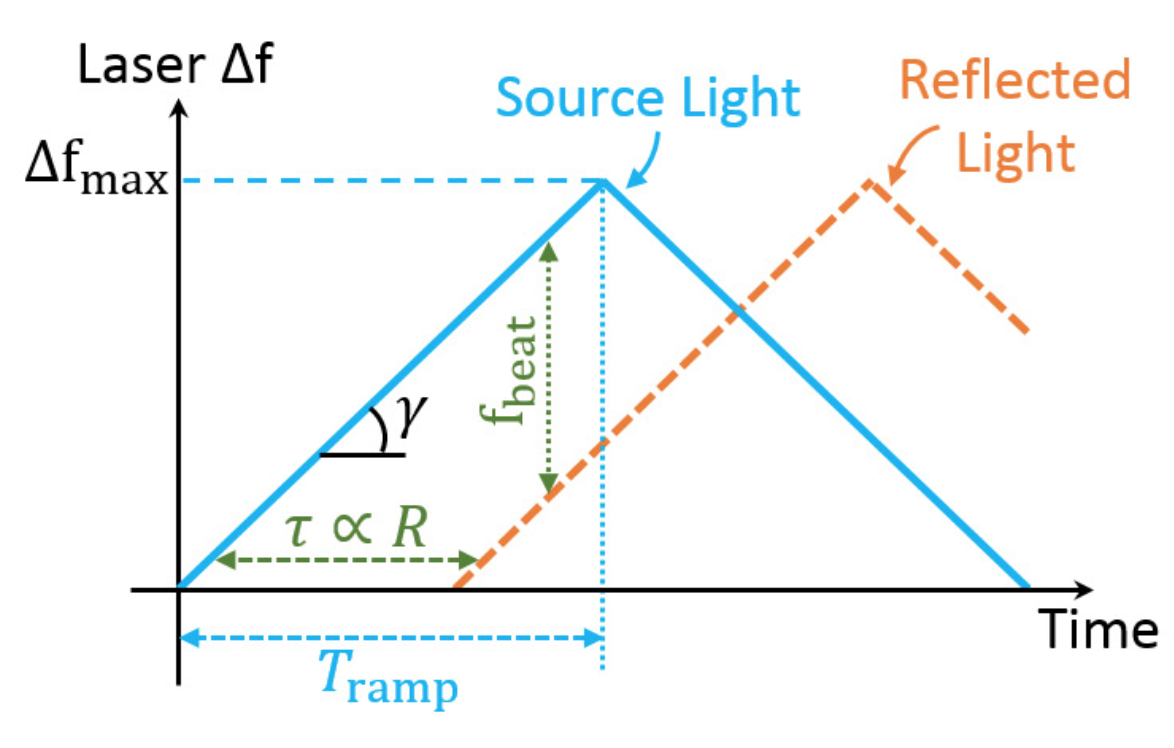
\includegraphics[width=0.5\columnwidth]{figure3}
\caption{Modulation profile of FMCW lidar \cite{behnam}}
\vspace{-0.3in}
\label{lidarsignal}
\end{figure}


As seen from the numerical example in the previous section, solving semidefinite program for line spectral estimation is very expensive in terms of computation complexity (solving a problem of size 200 took almost a minute). Let's see what is the actual size of the sample data in typical lidar system.

Fig. \ref{lidarsignal} \cite{behnam} shows the laser frequency modulation waveform for FMCW lidar (triangular pattern). Typical values of the parameters in this profile for real-world application is as follows.

\begin{itemize}
    \item Desired maximum distance range ($d_{max}$): $10m$
    \item Chirping bandwidth ($\Delta f_{max}$): $10GHz$
    \item Pixel observation window ($T_{ramp}$): $10\mu s$
    \item Chirping rate ($\gamma=\Delta f_{max}/T_{ramp}$): $1PHz/s$
    \item Maximum beating frequency ($f_{beat,max} = 2\gamma d_{max}/c$): $66.7MHz$
    \item Required sampling rate ($f_{sample} = 2f_{beat,max}$): $133MHz$
    \item Number of samples in the time domain ($N_{sample} = T_{obs}f_{sample}$): $1,330$
\end{itemize}

\noindent This shows that the typical size of the problem is $N=1,000\sim10,000$, and it is clear that full-blown semidefinite approach is not an option.

There are two potential approaches for problem simplification. First, we introduced the dual problem formulated as semidefinite program as the original problem was defined in the continuous domain with infinite dimension, and it was impossible to solve such problem numerically. We can still discretize the support space (frequency domain), and the size of that discrete grid is going to be determined by the trade-off between complexity and the resolving power beyond the resolution limit (or super-resolution factor SRF). Then the problem is now formulated on a finite field and the problem size is now $SRF \times N$. There are plenty of $l1$ minimization algorithms, and one of them could potentially show the best performance for given complexity constraint.

Secondly, we can leverage the fact that it is almost always the case that the lidar signal contains only one non-zero tone (or two non-zero tones with complement amplitudes). Multi-path propagation path from the transmitter to receiver is very unlikely since the beamforming antenna for integrated lidar system generally has extremely high directivity \cite{yaacobi}. This introduces another constraint for the original optimization problem, and reduces the size of the optimization space.

\begin{equation}
    \min_{ \tilde{x} }{\| \tilde{x} \|_{1}} \quad \textrm{subject to} \quad \| \tilde{x} \|_0 = 1 \textrm{ and } \| \mathcal{F}_n \tilde{x} - y \|_2 \leq \delta
\end{equation}

There are $SRF \times N$ supports in the optimization space, and we can parallelize the search process of finding the amplitude of minimum magnitude that still satisfies $\| \mathcal{F}_n \tilde{x} - y \|_2 \leq \delta$. After that process, one can simply pick the support with smallest magnitude. 

%Fig. \ref{diephoto}(a) shows the die photo of the MPC equalizer chip, which was fabricated in 28nm FDSOI CMOS. A 3-bit core for PAM2 and \textit{two-eye} modulation, and a 4-bit core for PAM4 modulation were implemented. The final DAC was implemented using a segmented voltage-mode driver (Fig. \ref{diephoto}(b)) matched to 50$\Omega$ when all segments are enabled. To avoid the nonlinearity inherent in this DAC, we used 32 segments, more than actual signal level and a lookup table to map the MPC solution to the number of ``on'' segments (resulting on-segment vs. output level plot is shown in Fig. \ref{diephoto}(c)). The total swing of the transmitter when loaded by the 50$\Omega$ termination is 462$\textrm{mV}_{\textrm{pp}}$.

%To demonstrate equalizer performance with a reflective multidrop channel, the chip was connected to an oscilloscope through two series connected 8-inch differential copper traces with two stubs and 3m of coaxial cable. The pulse response and normalized tap coefficients of the entire channel at 4.5GBaud/s is shown in Fig. \ref{impulse}(a). Indeed, this channel is corrupted by reflection due to the impedance mismatch from the via stubs, and the eye for PAM2 modulated data with a 4.5Gb/s PRBS31 sequence is completely closed (Fig. \ref{impulse}(b)). By activating MPC equalization in the 3-bit core, the eye is fully open in PAM2 mode (Fig. \ref{eyes}(a)). The \textit{two-eye} mode shows similar performance (Fig. \ref{eyes}(b)). 

%\begin{figure}[t!]
%\centering
%%\vspace{-0.1in}
%\includegraphics[width=0.95\columnwidth]{impulse}
%\caption{(a) Impulse response of the channel at 4.5GBaud/s and (b) unequalized eye (PAM2)}
%\vspace{-0.16in}
%\label{impulse}
%\end{figure}

%\vspace{-0.2in}
%\begin{figure}[t!]
%\centering
%%\vspace{-0.1in}
%\includegraphics[width=0.95\columnwidth]{eyes}
%\caption{MPC-equalized eye for (a) PAM2 and (b) two-eye modulation at 4.5Gb/s, and (c) un-equalized/(d) equalized eye for PAM4 at 6Gb/s, all with PRBS31 sequence}
%\vspace{-0.3in}
%\label{eyes}
%\end{figure}

%With 1V supply, The 3-bit core consumes 1.33pJ/b at 4.5Gb/s with all of the FIR taps turned off. The power consumption within the FIR is determined by the activity factor, and as a result scales roughly linearly with the number of active taps and the tap weights for the channel. In order to increase the tap weight by 10\% of the main tap, the 3-bit core was measured to consume extra 0.2pJ/b at 4.5Gb/s. For our channel example (Fig. \ref{impulse}(a)), the sum of total postcursor weights compared to the main tap was around 100\% and the resulting equalizer energy efficiency was 3.33pJ/b. As shown in Table \ref{tbl1}, this is similar to the efficiency of the latest THP transmitter demonstration, despite the difference in technology and the fact that THP demonstration utilized customized arithmetic elements tailored for that algorithm. Since the entire architecture is purely digital, we can expect direct improvements in efficiency and data-rate for newer technologies.
%The 3-bit core is capable of equalizing the multidrop channel at 5Gb/s, albeit at a lower energy efficiency of 5.88pJ/bit due to a supply voltage increase to 1.2V. 

%By using the 4-bit core we can also perform PAM4 modulation (Fig. \ref{eyes}(d)) at 6Gb/s with a total power consumption of 5.8pJ/b using the same channel. This increase in power comes primarily because of the larger search space and tap unrolling blocks due to the increased resolution.

\section{Conclusion}

In this report, different line-spectral support recovery schemes are examined for FMCW lidar receiver with both closed-form expressions for the estimation error and numerical examples. Especially, it was confirmed that convex optimization-based super-resolution receiver achieves much superior detection performance even in rather low-SNR regime, well within the resolution limit. At the same time, we realized that the original problem formulation is not suitable for latency-critical lidar sensor due to its high complexity. I also proposed possible strategies to used super-resolution detector in the lidar system by leveraging the nature of lidar signal. In following work, I will examine the performance of proposed discretized-support, 0-norm constraint optimization-based support recovery. 
%\vspace{0.5em}
%A Model Predictive Control transmitter is demonstrated in a 28nm FDSOI process as a new, fully-digital TX equalization algorithm for high-speed I/Os in asymmetric environments. It is shown that the MPC can achieve better eye performance compared to other schemes such as THP, especially when the equalization hardware uses only a few bits to represent the control signal. In addition, with MPC, the overhead (number of slicers and decoding) at the receiver side is determined only by the modulation scheme and not by the channel characteristic.

%The DS MPC algorithm, a simplified MPC leveraging resolution insensitivity, is used to implement a high-speed transmit equalizer with a series of micro-achitectural optimizations. For highly reflective channel multidrop channel example, the MPC chip opens up the closed eye for 4.5Gb/s PAM2 and 6Gb/s PAM4 with similar efficiency as the latest THP demonstration \cite{THP}. Considering that this prototype chip was synthesized directly from RTL and the system complexity is actually lower, we expect that the MPC can achieve much better performance and efficiency when realized with customized arithmetic blocks in the latest technology node.

%\begin{table}[!t]
%\renewcommand{\arraystretch}{1.5}
%\caption{\textsc{Comparison of Equalizers for Memory I/O Links}}
%\label{tbl1}
%\centering
%\begin{tabular}[c]{ 
%@{ { }}m{0.25\columnwidth} >{\centering}m{0.15\columnwidth} @{ { }} >{\centering}m{0.15\columnwidth} @{ { }} >{\centering}m{0.15\columnwidth}@{} @{ { }} >{\centering}m{0.15\columnwidth}@{}}
%\hthickline 
 %&\cite{THP}&\cite{duobinary}&\cite{multitone}&\textbf{This work\\(3bit/4bit)}  \tabularnewline \hthickline 
%Process [nm] & 22 & 45 & 40 & \textbf{28}  \tabularnewline\hline
%Data Rate [Gb/s] & 10 & 5.8 & 7.5 & \textbf{4.5/6}\tabularnewline\hline
%Algorithm & THP & DFE & -- & \textbf{MPC} \tabularnewline\hline
%No. of taps  & 8 & 7 & -- & \textbf{20}\tabularnewline\hline
%Modulation & PAM2/4 & Duobinary & Multi-tone\\PAM2 & \textbf{PAM2\\\textit{two-eye} / PAM4} \tabularnewline\hline
%Efficiency [pJ/b] & 1.2 & 2.45 & 1 & \textbf{1.33/3.2}\tabularnewline\hline
%Extra Power for 10\% Main Tap Compensation [pJ/b/tap]& 0.14 & -- & -- & \textbf{0.2/0.371}  \tabularnewline\hline
%Area [mm${}^\textrm{2}$] & 0.019 & 0.087 & 0.015 & \textbf{0.023/0.053}\tabularnewline\hthickline
%\end{tabular}
%\vspace{-1.5em}
%\end{table}
%\vspace{-1em}



%\section*{Acknowledgment}
%\vspace{0.5em}
%This work was supported in part by the fabrication donation from STMicroelectronics, and in part by the DARPA POEM Award HR0011-11-C-0100 and contract HR0011-11-9-0009, and in part by Berkeley Wireless Research Center, Trusted Foundry, and the Kwanjeong Educational Foundation.
%We acknowledge the help of Amr Suleiman of MIT, Ranko Sredojevi\'{c}, Sen Lin, Sajjad Moazeni and Nandish Mehta of University of California, Berkeley.



% An example of a floating figure using the graphicx package.
% Note that \label must occur AFTER (or within) \caption.
% For figures, \caption should occur after the \includegraphics.
% Note that IEEEtran v1.7 and later has special internal code that
% is designed to preserve the operation of \label within \caption
% even when the captionsoff option is in effect. However, because
% of issues like this, it may be the safest practice to put all your
% \label just after \caption rather than within \caption{}.
%
% Reminder: the "draftcls" or "draftclsnofoot", not "draft", class
% option should be used if it is desired that the figures are to be
% displayed while in draft mode.
%
%\begin{figure}[!t]
%\centering
%\includegraphics[width=2.5in]{myfigure}
% where an .eps filename suffix will be assumed under latex, 
% and a .pdf suffix will be assumed for pdflatex; or what has been declared
% via \DeclareGraphicsExtensions.
%\caption{Simulation Results}
%\label{fig_sim}
%\end{figure}

% Note that IEEE typically puts floats only at the top, even when this
% results in a large percentage of a column being occupied by floats.


% An example of a double column floating figure using two subfigures.
% (The subfig.sty package must be loaded for this to work.)
% The subfigure \label commands are set within each subfloat command, the
% \label for the overall figure must come after \caption.
% \hfil must be used as a separator to get equal spacing.
% The subfigure.sty package works much the same way, except \subfigure is
% used instead of \subfloat.
%
%\begin{figure*}[!t]
%\centerline{\subfloat[Case I]\includegraphics[width=2.5in]{subfigcase1}%
%\label{fig_first_case}}
%\hfil
%\subfloat[Case II]{\includegraphics[width=2.5in]{subfigcase2}%
%\label{fig_second_case}}}
%\caption{Simulation results}
%\label{fig_sim}
%\end{figure*}
%
% Note that often IEEE papers with subfigures do not employ subfigure
% captions (using the optional argument to \subfloat), but instead will
% reference/describe all of them (a), (b), etc., within the main caption.


% An example of a floating table. Note that, for IEEE style tables, the 
% \caption command should come BEFORE the table. Table text will default to
% \footnotesize as IEEE normally uses this smaller font for tables.
% The \label must come after \caption as always.
%
%\begin{table}[!t]
%% increase table row spacing, adjust to taste
%\renewcommand{\arraystretch}{1.3}
% if using array.sty, it might be a good idea to tweak the value of
% \extrarowheight as needed to properly center the text within the cells
%\caption{An Example of a Table}
%\label{table_example}
%\centering
%% Some packages, such as MDW tools, offer better commands for making tables
%% than the plain LaTeX2e tabular which is used here.
%\begin{tabular}{|c||c|}
%\hline
%One & Two\\
%\hline
%Three & Four\\
%\hline
%\end{tabular}
%\end{table}


% Note that IEEE does not put floats in the very first column - or typically
% anywhere on the first page for that matter. Also, in-text middle ("here")
% positioning is not used. Most IEEE journals/conferences use top floats
% exclusively. Note that, LaTeX2e, unlike IEEE journals/conferences, places
% footnotes above bottom floats. This can be corrected via the \fnbelowfloat
% command of the stfloats package.



% conference papers do not normally have an appendix

% use section* for acknowledgement

% the Defense Advanced
%Research Projects Agency (DARPA) of the United States
%under the E-PHI project, grant no. HR0011-12-2-0007 and
%DARPA MTO Program Manager Dr. Josh Conway and also in
%part by W911NF-12-1-0210 under Dr. Jag Shah.


% trigger a \newpage just before the given reference
% number - used to balance the columns on the last page
% adjust value as needed - may need to be readjusted if
% the document is modified later
%\IEEEtriggeratref{8}:
% The "triggered" command can be changed if desired:
%\IEEEtriggercmd{\enlargethispage{-5in}}

% references section

% can use a bibliography generated by BibTeX as a .bbl file
% BibTeX documentation can be easily obtained at:
% http://www.ctan.org/tex-archive/biblio/bibtex/contrib/doc/
% The IEEEtran BibTeX style support page is at:
% http://www.michaelshell.org/tex/ieeetran/bibtex/
%\bibliographystyle{IEEEtran}
% argument is your BibTeX string definitions and bibliography database(s)
%\bibliography{IEEEabrv,../bib/paper}
%
% <OR> manually copy in the resultant .bbl file
% set second argument of \begin to the number of references
% (used to reserve space for the reference number labels box)
\bibliographystyle{IEEEtran}
\bibliography{reference}




% that's all folks
\end{document}


